\documentclass{article}
\usepackage{url}
\usepackage{color}
\usepackage{amsfonts,amssymb,latexsym,theorem}
\usepackage{a4wide}
\usepackage{graphicx}

\def\at#1#2{{\char64}_{#1}#2}
\newbox\itembox
\def\itemlistlabel#1{#1\hfill}
\def\itemlist#1{\setbox\itembox=\hbox{#1}%
		\list{}{\labelwidth\wd\itembox
		             \leftmargin\labelwidth
                             \advance\leftmargin by\itemindent
			     \advance\leftmargin by\labelsep
			      \let\makelabel\itemlistlabel}}
\let\enditemlist\endlist
\def\Mseq#1#2#3{{#1}_{1},...,{#1}_{#2}\in #3}
\def\Mseqc#1#2{{#1}_{1}\wedge\cdots\wedge{#1}_{#2}}


\def\goth#1{\mathfrak{#1}}
\def\gothA{{\mathfrak{A}}}			\def\gotha{{\mathfrak{a}}}
\def\gothB{{\mathfrak{B}}}			\def\gothb{{\mathfrak{b}}}
\def\gothC{{\mathfrak{C}}}			\def\gothc{{\mathfrak{c}}}
\def\gothD{{\mathfrak{D}}}			\def\gothd{{\mathfrak{d}}}
\def\gothE{{\mathfrak{E}}}			\def\gothe{{\mathfrak{e}}}
\def\gothF{{\mathfrak{F}}}			\def\gothf{{\mathfrak{f}}}
\def\gothG{{\mathfrak{G}}}			\def\gothg{{\mathfrak{g}}}
\def\gothH{{\mathfrak{H}}}			\def\gothh{{\mathfrak{h}}}
\def\gothI{{\mathfrak{I}}}			\def\gothi{{\mathfrak{i}}}
\def\gothJ{{\mathfrak{J}}}			\def\gothj{{\mathfrak{j}}}
\def\gothK{{\mathfrak{K}}}			\def\gothk{{\mathfrak{k}}}
\def\gothL{{\mathfrak{L}}}			\def\gothl{{\mathfrak{l}}}
\def\gothM{{\mathfrak{M}}}			\def\gothm{{\mathfrak{m}}}
\def\gothN{{\mathfrak{N}}}			\def\gothn{{\mathfrak{n}}}
\def\gothO{{\mathfrak{O}}}			\def\gotho{{\mathfrak{o}}}
\def\gothP{{\mathfrak{P}}}			\def\gothp{{\mathfrak{p}}}
\def\gothQ{{\mathfrak{Q}}}			\def\gothq{{\mathfrak{q}}}
\def\gothR{{\mathfrak{R}}}			\def\gothr{{\mathfrak{r}}}
\def\gothS{{\mathfrak{S}}}			\def\goths{{\mathfrak{s}}}
\def\gothT{{\mathfrak{T}}}			\def\gotht{{\mathfrak{t}}}
\def\gothU{{\mathfrak{U}}}			\def\gothu{{\mathfrak{u}}}
\def\gothV{{\mathfrak{V}}}			\def\gothv{{\mathfrak{v}}}
\def\gothW{{\mathfrak{W}}}			\def\gothw{{\mathfrak{w}}}
\def\gothX{{\mathfrak{X}}}			\def\gothx{{\mathfrak{x}}}
\def\gothY{{\mathfrak{Y}}}			\def\gothy{{\mathfrak{y}}}
\def\gothZ{{\mathfrak{Z}}}			\def\gothz{{\mathfrak{z}}}

\def\calA{{\cal A}}			\def\cA{{\cal a}}
\def\calB{{\cal B}}			\def\cb{{\cal b}}
\def\calC{{\cal C}}			\def\calc{{\cal c}}
\def\calD{{\cal D}}			\def\cd{{\cal d}}
\def\calE{{\cal E}}			\def\ce{{\cal e}}
\def\calF{{\cal F}}			\def\cf{{\cal f}}
\def\calG{{\cal G}}			\def\cg{{\cal g}}
\def\calH{{\cal H}}			\def\ch{{\cal h}}
\def\calI{{\cal I}}			\def\ci{{\cal i}}
\def\calJ{{\cal J}}			\def\cj{{\cal j}}
\def\calK{{\cal K}}			\def\ck{{\cal k}}
\def\calL{{\cal L}}			\def\cl{{\cal l}}
\def\calM{{\cal M}}			\def\cm{{\cal m}}
\def\calN{{\cal N}}			\def\cn{{\cal n}}
\def\calO{{\cal O}}			\def\co{{\cal o}}
\def\calP{{\cal P}}			\def\cp{{\cal p}}
\def\calQ{{\cal Q}}			\def\cq{{\cal q}}
\def\calR{{\cal R}}			\def\calr{{\cal r}}
\def\calS{{\cal S}}			\def\cs{{\cal s}}
\def\calT{{\cal T}}			\def\ct{{\cal t}}
\def\calU{{\cal U}}			\def\cu{{\cal u}}
\def\calV{{\cal V}}			\def\cv{{\cal v}}
\def\calW{{\cal W}}			\def\cw{{\cal w}}
\def\calX{{\cal X}}			\def\cx{{\cal x}}
\def\calY{{\cal Y}}			\def\cy{{\cal y}}
\def\calZ{{\cal Z}}			\def\cz{{\cal z}}

\def\sfA{{\sf A}}			\def\sfa{{\sf a}}
\def\sfB{{\sf B}}			\def\sfb{{\sf b}}
\def\sfC{{\sf C}}			\def\sfc{{\sf c}}
\def\sfD{{\sf D}}			\def\sfd{{\sf e}}
\def\sfE{{\sf E}}			\def\sfe{{\sf f}}
\def\sfF{{\sf F}}			\def\sff{{\sf f}}
\def\sfG{{\sf G}}			\def\sfg{{\sf g}}
\def\sfH{{\sf H}}			\def\sfh{{\sf h}}
\def\sfI{{\sf I}}			\def\sfi{{\sf i}}
\def\sfJ{{\sf J}}			\def\sfj{{\sf j}}
\def\sfK{{\sf K}}			\def\sfk{{\sf k}}
\def\sfL{{\sf L}}			\def\sfl{{\sf l}}
\def\sfM{{\sf M}}			\def\sfm{{\sf m}}
\def\sfN{{\sf N}}			\def\sfn{{\sf n}}
\def\sfO{{\sf O}}			\def\sfo{{\sf o}}
\def\sfP{{\sf P}}			\def\sfp{{\sf p}}
\def\sfQ{{\sf Q}}			\def\sfq{{\sf q}}
\def\sfR{{\sf R}}			\def\sfr{{\sf r}}
\def\sfS{{\sf S}}			\def\sfs{{\sf s}}
\def\sfT{{\sf T}}			\def\sft{{\sf t}}
\def\sfU{{\sf U}}			\def\sfu{{\sf u}}
\def\sfV{{\sf V}}			\def\sfv{{\sf v}}
\def\sfW{{\sf W}}			\def\sfw{{\sf w}}
\def\sfX{{\sf X}}			\def\sfx{{\sf x}}
\def\sfY{{\sf Y}}			\def\sfy{{\sf y}}
\def\sfZ{{\sf Z}}			\def\sfz{{\sf z}}

\def\forces{\models}
\def\univ{\mathrm{E}}
\def\Univ{\mathrm{A}}
\newcommand{\lgcof}[1]{\Lambda_{#1}}
\newcommand{\mcs}{\textsc{mcs}}

\title{\textsf{Curso: Generaci\'on de Lenguaje Natural y Aplicaciones}\\
Escuela de Ling\"u\'istica Computacional 2010 \\
26-31 de Julio 2010, Buenos Aires, Argentina\\
}
\author{Evaluaci\'on Take Home}
\date{Entrega: \textbf{Lunes 16 de Agosto, 2010}\\
\mbox{    } }

\begin{document}

\maketitle



\textbf{Pregunta 1: } 
\begin{enumerate}
\item Enumerar las etapas b\'asicas de un sistema estandar 
de GLN, describiendo cada una de ellas en 2 renglones. 
\item Muchos sistemas organizan
estas etapas en un pipeline. 
\begin{enumerate}
\item Describir las \textbf{desventajas} de esta 
arquitectura (max 5 renglones).  

\item Mencionar expl\'icitamente dos etapas donde la arquitectura 
pipeline es particularmente problem\'atica y dar un ejemplo de generaci\'on 
concreto donde la calidad del texto mejorar\'ia al no usar un pipeline. 
  
\end{enumerate}
\end{enumerate}

\medskip
\textbf{Pregunta 2: } 
Considerar la siguiente gram\'atica l\'exica TAG presentada en clase

\begin{center}
\framebox{
\begin{minipage}{.8\textwidth}
\begin{center}
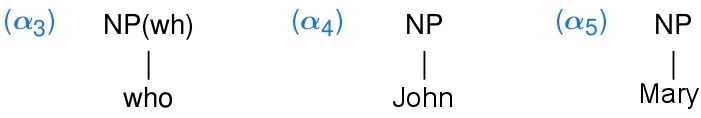
\includegraphics[scale=.45]{slides/pics/pic2-30.jpg} 
\medskip

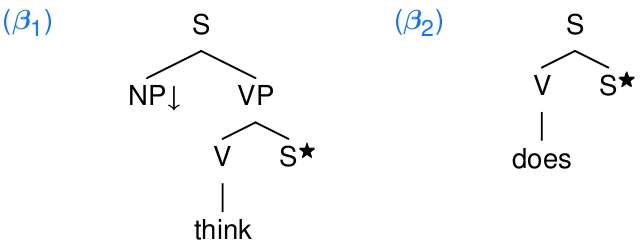
\includegraphics[scale=.45]{slides/pics/pic2-29.jpg} 
\medskip

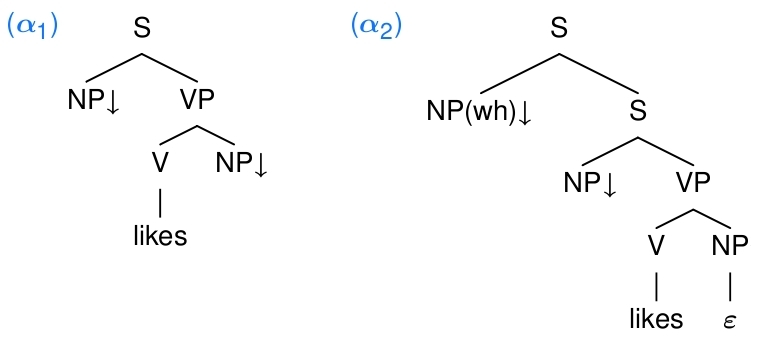
\includegraphics[scale=.45]{slides/pics/pic2-28.jpg}
\end{center}
\end{minipage}}
\end{center}

\begin{enumerate}
\item Mostrar que la frase ``Who does John think Mary likes'' pertenece al lenguaje 
de la gram\'atica, mostrando los distintos pasos de la construcci\'on del \'arbol. 

\item Dar tres ejemplos de frases generadas por la gram\'atica que no son gramaticalmente 
correctas\footnote{Cualquier noci\'on razonable de `gramaticalidad' est\'a bien, no vamos 
a ser estrictos con eso. Pero intenten que los ejemplos sean lo mas diferente posible entre 
ellos.}.

\item Dar una descripci\'on, lo m\'as detallada posible, de las frases generadas por 
la gram\'atica. 

\item Si restringimos las operaciones de sustitucion y adjuncci\'on de forma que no permitimos 
sustituciones una vez que una operaci\'on de adjuncci\'on ha sido aplicada, obtenemos el mismo 
lenguaje? Justifique por que. 
\end{enumerate}

\medskip
\textbf{Pregunta 3:} El algoritmo incremental de Dale and Reiter para la GRE puede definirse
de la siguiente forma:

\begin{center}
\framebox{
\begin{minipage}{.8\textwidth}
\begin{description}
\item[Input:] \ \\
            Un conjunto de individuos con sus propiedades\\
            Un individuo target. 
\item[Output:] \ \\
            Un conjunto de propiedades
\item[Algoritmo:] \ \\
            Empezar con un conjunto vac\'io\\
            Agregar propiedades del objeto target, mientras cada propiedad elimine al menos a un distractor 
y mientras el conjunto de distractores sea no vac\'io.
\end{description}
\end{minipage}}
\end{center}

Asumamos que en cada iteraci\'on, la propiedad a utilizar se elige en forma `greedy' utilizando aquella con 
mayor poder discriminatorio.  

\begin{enumerate}
\item Dar un ejemplo de un conjunto de objetos y propiedades donde para alg\'un objeto 
target, la heur\'istica greedy no lleva a la descripci\'on m\'as corta. 
\item Extender el algoritmo para que tome un orden parcial sobre las propiedades y proponer combinaciones 
de este orden con el poder discriminatorio de una propiedad.  Dar ejemplos. 
\end{enumerate}

\medskip
\textbf{Pregunta 4: } 
\begin{enumerate}

\item \textbf{Monos y Bananas:} un mono esta en una habitaci\'on con unas bananas 
colgando del techo.  La habitaci\'on tiene una caja a la que el mono puede 
subirse para alcanzar las bananas. Inicialmente, el mono esta en la posici\'on A, 
las bananas en la posici\'on B, y la caja en la posici\'on C. El mono y la caja 
tiene la propiedad `altura baja,' pero si el mono se sube a la caja, su 
altura pasa a ser `alta' que es la misma altura a la que est\'an las bananas. 
Las acciones que el mono puede realizar son \emph{Ir} de una posici\'on a otra. 
\emph{Empujar} un objeto de un lugar a otro.  \emph{TreparA} y \emph{BajarseDe}
un objeto. Y \emph{Tomar} y \emph{Soltar} un objeto. La acci\'on \emph{Tomar}
resulta en el objeto estando en posesi\'on del mono, siempre y cuando el mono 
y el objeto esten en el mismo lugar y a la misma altura. 

\begin{enumerate}
\item Especificar el estado inicial descripto, y un estado final en donde el 
mono tiene las bananas. 
\item Especificar las seis acciones mencionadas, usando STRIPS. 
\end{enumerate}

\newpage 
\item Considerar el siguiente problema de planning

\vspace*{-.2cm}
\begin{center}
\framebox{
\begin{minipage}{0.8\textwidth}
\begin{center}
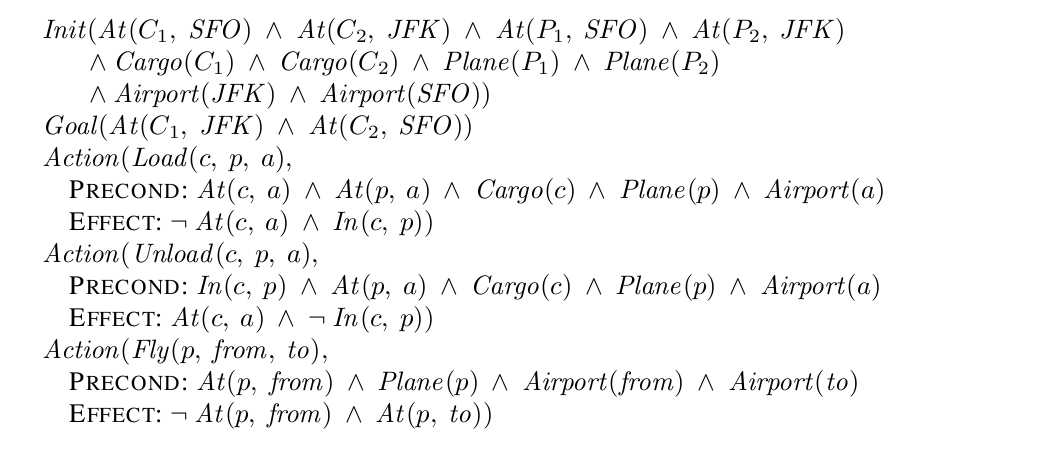
\includegraphics[scale=.5]{planning.jpg} 
\end{center}
\end{minipage}
}
\end{center}

\vspace*{-.2cm}
Construir los niveles 0, 1 y 2 del grafo de planning (graphplan) indicando mutexes. 

\item Demostrar la siguiente propiedad de un grafo de planning

\begin{quote}
Un literal que no aparece en el \'ultimo nivel de un grafo de planning (totalmente
expandido, i.e., cuando el grafo `leveled off') no puede ser alcanzado desde el estado inicial por ninguna secuencia de
acciones. 
\end{quote}
\end{enumerate}

\medskip
\textbf{Pregunta 5:} Durante el \'ultimo d\'ia de clase discutimos distintas 
m\'etricas que pueden utilizarse para evaluar la calidad de un sistema de 
generaci\'on de instrucciones en un ambiente virtual.  Supongamos que queremos 
evaluar (independientemente una de otra) las siguientes caracter\'isticas de un sistema
\begin{itemize}
   \item Eficiencia y eficacia\\[-2em]
   \item Entretenimiento\\[-2em]
   \item Generaci\'on de background com\'un entre el sistema y el usuario.  
\end{itemize}

Dar para cada caracter\'istica un listado ordenado 
de las m\'etricas `Top 5.' Es decir, mencionar en cada caso, en orden de mejor a 
peor, 5 m\'etricas que eval\'uan la caracter\'istica indicada.  Para cada una 
de las listas dadas, argumentar el orden elegido\footnote{Pueden incluir m\'etricas
no mencionadas en clase, argumentando c\'omo obtenerlas y por qu\'e son mejores que otras.}.    

\end{document}
